% CN: 熵正则 UOT、UFGW solver 和下游实验使用实测结果；各图表单独注明来源。
% EN: Entropic UOT, UFGW solver and downstream experiments use measurements, with sources recorded for each figure and table.
\subsection{Sparse Entropic UOT}
\label{sec:entropic-experiments}
% \xwz{RERUN REQUIRED FOR THE WEIGHT-BUDGET CHANGE: the historical entropic Pareto and epsilon-sweep records do not retain complete per-restricted-call restart counts or controller traces, so inactivity of the new J=64, p=1.01 budget cannot be certified. Rerun the SHUTTLE-dependent configurations with the protected controller, retaining the original precision and entropic objectives, and update Figure fig:entropic-runtime-accuracy and Appendix app:entropic-epsilon-accuracy. OTT/Spar-Sink measurements and independently audited reference bounds need not be rerun solely for this change. Audit: experiments/primal_weight_budget_20261111/report/history_J64_audit.json.}

We evaluate \ourssparsink against online \sinkhorn in OTT and the importance-sparsification method Spar-Sink.
We compare direct reuse of the final active support with support reconstruction that retains positive-flow edges and selects bidirectional top-$b_{\mathrm e}$ edges by the final unregularized dual scores.
Each comparison fixes the entropic strength $\varepsilon$ and marginal penalties, so every method approximates the same full entropic UOT problem.
We evaluate the full entropic primal objective $P_\varepsilon$, including the entropy constant outside the reported support, and use a shared dual lower bound $D_{\varepsilon,\mathrm{ref}}$ from an independent FP64 OTT-online solve with native stopping threshold $10^{-8}$:
\begin{equation}
\entropicgap=\frac{P_\varepsilon-D_{\varepsilon,\mathrm{ref}}}{\max\{|P_\varepsilon|,|D_{\varepsilon,\mathrm{ref}}|,10^{-15}\}}.
\label{eq:entropic-evaluation-gap}
\end{equation}
Runtime covers prepared CPU inputs through synchronized solver output, including input transfer, the unregularized \ours solve, support construction, and sparse refinement when used; compilation, warmup, and common post-solve evaluation are excluded.
Figure~\ref{fig:entropic-runtime-accuracy} compares runtime and approximation quality as each method's computational budget varies.
At $b_{\mathrm e}=8$, \ourssparsink achieves a shared gap below $5\times10^{-7}$ in all four penalty configurations, taking approximately $2$--$15$ seconds.
Increasing the support budget to $32$ reduces the gap below $10^{-10}$ in approximately $2$--$16$ seconds, whereas direct reuse yields gaps of approximately $3\times10^{-6}$--$6\times10^{-6}$.
% \xwz{The unmeasured Schmitzer/LCN appendix and its main-text promise are temporarily omitted.}
% Additional comparisons with Schmitzer's multiscale solver and LCN clustering with sparse \sinkhorn are deferred to Appendix~\ref{app:entropic-additional-baselines}.
% CN: epsilon 扫描来自 paper_experiments_uot/entropic_epsilon_accuracy/results/epsilon_sparse_log7_n16384_20261110_gpu267/summary.json，28/28成功，仅评估返回的 sparse coupling。
% EN: Epsilon-sweep results come from paper_experiments_uot/entropic_epsilon_accuracy/results/epsilon_sparse_log7_n16384_20261110_gpu267/summary.json, with 28/28 successful sparse-coupling evaluations.
A separate sweep with automatic support reconstruction gives shared gaps of $2.10$--$2.36\times10^{-7}$ and relative coupling $\ell_1$ errors of $9.31\times10^{-5}$--$1.99\times10^{-4}$ at $\varepsilon=10^{-3}$ across the four penalty settings.
Appendix~\ref{app:entropic-epsilon-accuracy} reports the full sweep and the reference coupling mass outside the reconstructed support.
% \xwz{If warm-start acceleration becomes a central claim, add a main-text comparison of cold-start and SHUTTLE--Sinkhorn-initialized full Sinkhorn, reporting end-to-end runtime including initialization as well as continuation iterations.}

\begin{figure}[t]
\centering
% CN: 图像来自 paper_experiments_uot/entropic_uot/results/20261026_225628_结果出来了_1e-3结果就很好了_后续使用rebuild会更好/entropic_uot_accuracy_runtime_pareto_2x2_eps0.001.png；数据为同目录 summary.csv，配置为 config.json 和 plot_selection.json。
% EN: Figure source: paper_experiments_uot/entropic_uot/results/20261026_225628_结果出来了_1e-3结果就很好了_后续使用rebuild会更好/entropic_uot_accuracy_runtime_pareto_2x2_eps0.001.png; data: summary.csv; settings: config.json and plot_selection.json in the same batch.
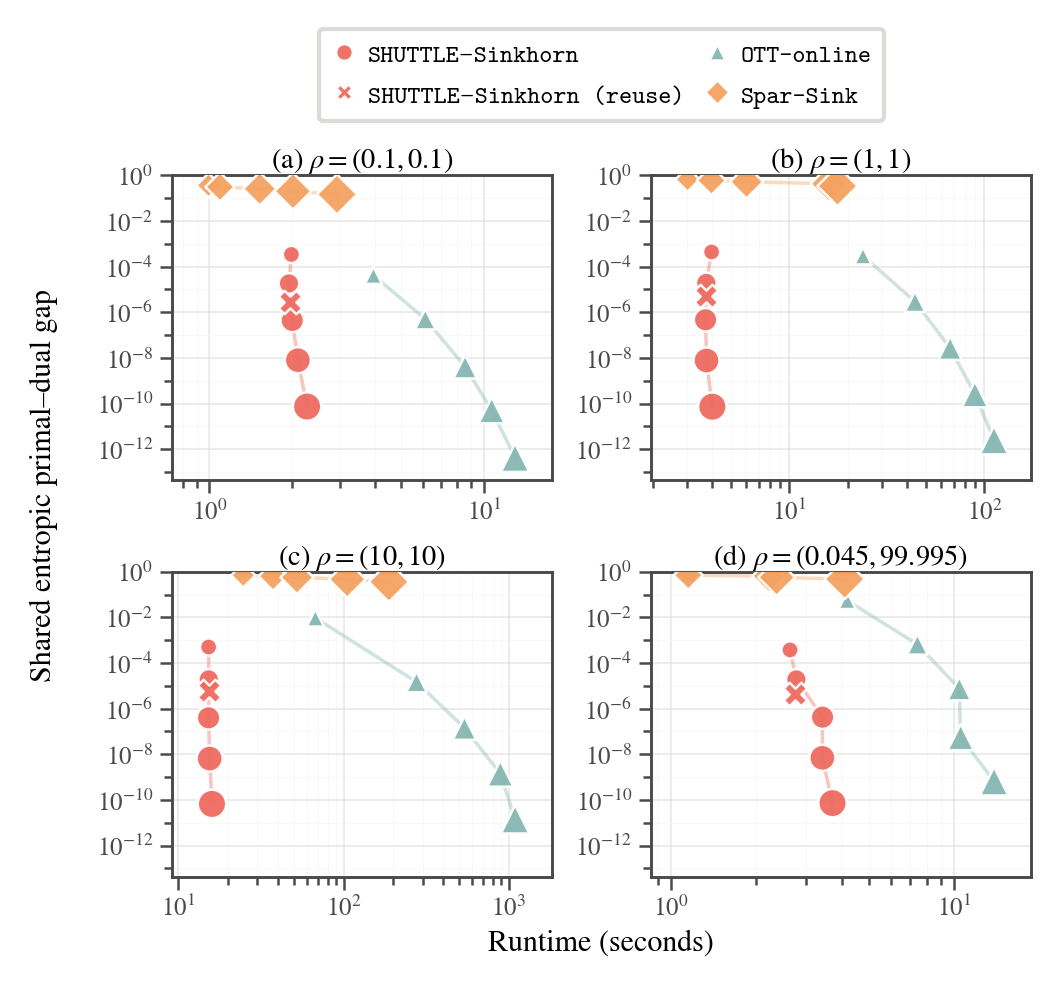
\includegraphics[width=\linewidth]{figures/entropic_uot_accuracy_runtime_pareto_eps0.001.png}
\caption{\textbf{Sparse entropic UOT runtime--accuracy comparison.}
TOME E11.5--E12.5 instances with $n=m=16{,}384$, $d=30$, and $\varepsilon=10^{-3}$.
Panels (a)--(d) use $(\rho_a,\rho_b)=(0.1,0.1),(1,1),(10,10),(0.045,99.995)$, respectively.
Connected points sweep the bidirectional support budget $b_{\mathrm e}\in\{2,4,8,16,32\}$ for \ourssparsink, the native stopping threshold from $10^{-2}$ to $10^{-6}$ for OTT-online, and the sampling budget factor from $8$ to $128$ for Spar-Sink; larger markers indicate larger budgets or tighter thresholds.
Crosses show direct support reuse.
The shared gap is defined in~\eqref{eq:entropic-evaluation-gap}.
Results use seed $42$ with one measurement per configuration.}
\label{fig:entropic-runtime-accuracy}
\end{figure}

\subsection{UFGW Solvers}
\label{sec:ufgw-experiments}

We compare two-coupling block-coordinate solvers on the same tensorized-KL UFGW formulation, using either \ours or POT to solve the UOT blocks.
At zero entropy, we compare \oursufgw with \bcdmm; with entropy, we compare \ourssinkhornufgw with \bcdsinkhorn, both BCD baselines using POT.
We denote the corresponding joint objective by \ufgwobj, with $\varepsilon=0$ recovering~\eqref{eq:ufgw-relaxation} and $\varepsilon>0$ using the regularized relaxation in Appendix~\ref{app:ufgw-extension}.
We match initialization, feature and structural costs, and penalty coefficients, and run exactly ten complete coupling-update sweeps with outer early stopping disabled.
Table~\ref{tab:ufgw-solvers} reports final objective values, runtime, and peak GPU memory on STARmap well05--well11.
At $\varepsilon=0$, \oursufgw is $28.1$ times faster than \bcdmm and attains a lower objective.
At $\varepsilon=10^{-3}$, \ourssinkhornufgw is $5.9$ times faster than \bcdsinkhorn, with final objectives differing by $2.1\times10^{-8}$.
Peak GPU memory is reduced from $40.02$ and $34.27$ GiB to $0.53$ GiB, respectively.
Appendix~\ref{app:ufgw-solver-trajectories} reports objective--time trajectories, and Appendix~\ref{app:implementation-ufgw} gives implementation and measurement details.

\begin{table}[t]
\centering
% CN: 四行实测结果来自 /home/xiawenzhou/project/hierarchical_ot/paper_experiments_uot/ufgw_solver_comparison/results/20261110_ufgw_starmap_n16384/{summary.json,summary.csv,cases/*/{shuttle,pot}_repeat0/metrics.json}；配置与输入指纹见同目录 config.json、manifest.json，4/4 成功，每组固定 10 个完整 P/Q sweeps。
% EN: All four measured rows come from /home/xiawenzhou/project/hierarchical_ot/paper_experiments_uot/ufgw_solver_comparison/results/20261110_ufgw_starmap_n16384/{summary.json,summary.csv,cases/*/{shuttle,pot}_repeat0/metrics.json}; config.json and manifest.json record settings and input fingerprints, with 4/4 successful fixed-budget runs of ten complete P/Q sweeps.
% \xwz{RERUN REQUIRED FOR THE WEIGHT-BUDGET CHANGE: SHUTTLE UFGW records lack complete restart-count evidence for their inner UOT calls. Rerun both SHUTTLE rows with J=64, p=1.01 and refresh the linked trajectories in Appendix UFGW Solver Trajectories; retain the declared ten-sweep protocol. POT baselines are unaffected by this controller change. Audit: experiments/primal_weight_budget_20261111/report/history_J64_audit.json.}
% CN: Time 使用 runtime_sec；Memory 使用 peak_gpu_memory_mib/1024 转为 GiB；objective 为共同 CPU FP64 目标，含 joint entropy 常数；加速比按未舍入耗时计算，不跨 epsilon 比较目标值。
% EN: Time uses runtime_sec; Memory converts peak_gpu_memory_mib to GiB by division by 1024; objectives use the common CPU FP64 evaluator including joint-entropy constants; speedups use unrounded times, without comparing objectives across epsilon settings.
% CN: Objective 保留五位小数；同一 epsilon 内按展示精度并列最好的目标值均加粗。
% EN: Objectives are rounded to five decimal places; tied best displayed objectives within each epsilon group are all bolded.
\caption{\textbf{UFGW solver comparison.}
STARmap well05--well11 with $m=n=16{,}384$, physical spatial coordinates, 30-dimensional expression features, $\alpha=0.4$, and $\rho_a=\rho_b=0.1$.
Both methods run ten complete sweeps from product couplings on A100 GPUs.
Time is in seconds and memory in GiB; common FP64 objective evaluation is excluded from timing.
Bold marks the best values within each entropy setting, including ties at the displayed precision.
Results use seed $0$ with one measurement per configuration.}
\label{tab:ufgw-solvers}
\footnotesize
\setlength{\tabcolsep}{2pt}
\begin{tabular}{@{}clrrr@{}}
\toprule
$\varepsilon$ & Method & \runtime~$\downarrow$ & \gpumemshort~$\downarrow$ & \ufgwobj~$\downarrow$ \\
\midrule
\multirow{2}{*}{$0$} & \bcdmm & 513.38 & 40.02 & 0.1113 \\
 & \oursufgw & \textbf{18.30} & \textbf{0.53} & \textbf{0.1110} \\
\midrule
\multirow{2}{*}{$10^{-3}$} & \bcdsinkhorn & 103.44 & 34.27 & \textbf{0.1222} \\
 & \ourssinkhornufgw & \textbf{17.64} & \textbf{0.53} & \textbf{0.1222} \\
\bottomrule
\end{tabular}

\end{table}

\subsection{Downstream Applications}
\label{sec:downstream-applications}

\paragraph{Temporal transport.}
% \xwz{RERUN REQUIRED FOR THE WEIGHT-BUDGET CHANGE: the archived SHUTTLE temporal results do not provide complete per-call restart counts across all time pairs, so unchanged behavior under J=64, p=1.01 cannot be established. Rerun the SHUTTLE--Sinkhorn configurations and update the linked temporal figures and timing breakdown; keep historical provenance and the authors' per-pair penalties. Full-rank and low-rank baselines are unaffected by this controller change. Audit: experiments/primal_weight_budget_20261111/report/history_J64_audit.json.}
Following the moscot temporal mapping benchmark~\citep{klein2025mapping}, we infer developmental transitions between adjacent mouse embryogenesis time points using the released 30-dimensional expression embeddings, growth priors, and downstream evaluation pipeline.
We compare full-rank \sinkhorn, \ourssparsink, and low-rank UOT~\citep{scetbon2023unbalanced} with ranks $10$, $100$, $1000$, and $2000$.
\ourssparsink reconstructs support within the final active-support budget and retains the resulting sparse coupling for downstream evaluation.
Full-rank \sinkhorn and \ourssparsink use $\varepsilon=0.005$ and matched marginal penalties; low-rank UOT follows the authors' separate rank-specific settings with $\varepsilon=10^{-4}$ and $1000$ iterations.
The marginal penalties vary across time pairs according to the authors' calibration of predicted apoptosis rates, so the comparison evaluates downstream utility under the published application settings.

% CN: 数值来自 paper_experiments_uot/moscot_time/results/20261102_005354_paper_data/{summary.csv,summary_table.csv}，114/114 项已完成；加速比按同一时间对的 coupling_evaluation_sec 相除，含 coupling 与 evaluation。
% EN: Numbers come from paper_experiments_uot/moscot_time/results/20261102_005354_paper_data/{summary.csv,summary_table.csv}, with 114/114 configurations complete; speedups divide paired coupling_evaluation_sec values, including coupling computation and evaluation.
Figure~\ref{fig:temporal-runtime} compares end-to-end time, curated transition accuracy (\transitionacc), and germ-layer accuracy.
Including both coupling computation and downstream evaluation, \ourssparsink achieves $3.44$--$217.58\times$ speedups over full-rank \sinkhorn and $1.83$--$18.11\times$ over low-rank UOT across all tested ranks and time pairs.
Appendix~\ref{app:temporal-timing} reports the coupling computation and evaluation times separately.
Across all 19 time pairs, the relative deviations of \ourssparsink from \sinkhorn are below $1.26\%$ for \transitionacc\ and $0.034\%$ for germ-layer accuracy, where relative deviation is the absolute score difference divided by the full-rank score.
The mean absolute difference in \transitionacc\ is $0.21$ percentage points, compared with $2.85$ and $2.03$ for low-rank ranks $1000$ and $2000$.
For each tested rank, \ourssparsink achieves higher \transitionacc\ on 16 of the 19 time pairs, consistently retaining accuracy close to full-rank \sinkhorn as runtime and low-rank approximation errors grow at later stages.

\begin{figure}[t]
\centering
% CN: 三联图来自 paper_experiments_uot/moscot_time/results/20261102_005354_paper_data/temporal_runtime_accuracy.pdf；数据为同目录 summary.csv、summary_table.csv；114/114 已完成。
% EN: Triptych source: paper_experiments_uot/moscot_time/results/20261102_005354_paper_data/temporal_runtime_accuracy.pdf; data: summary.csv and summary_table.csv in the same batch; 114/114 complete.
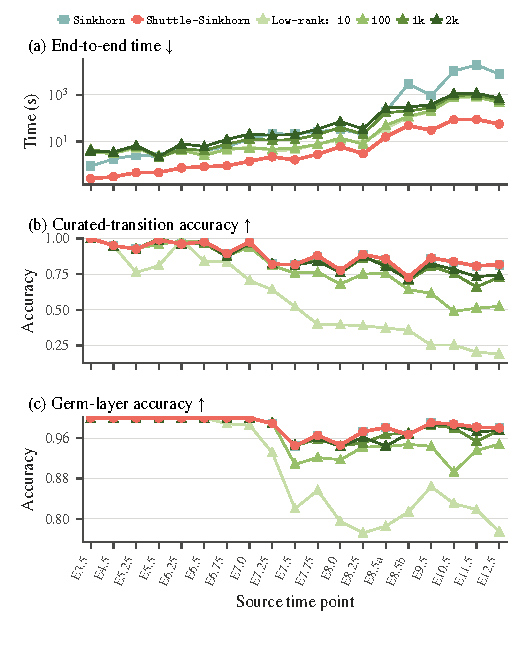
\includegraphics[width=\linewidth]{figures/moscot_time_runtime_accuracy.pdf}
\caption{\textbf{Temporal transport: runtime and downstream accuracy.}
(a) Coupling computation plus downstream evaluation time; (b) curated transition accuracy; (c) germ-layer accuracy.
\ourssparsink provides end-to-end speedups of up to $217.6\times$ over full-rank \sinkhorn and $18.1\times$ over low-rank UOT.
Triangle labels denote low-rank ranks ($1\mathrm{k}=1000$).
Time uses a logarithmic axis; accuracy axes are scaled independently.
Full-rank \sinkhorn is a computational reference rather than biological ground truth.
Results cover all 19 time pairs, using seed $42$ with one measurement per configuration on A100 GPUs.}
\label{fig:temporal-runtime}
\label{fig:temporal-accuracy}
\end{figure}

\paragraph{Spatial alignment.}
% \xwz{RERUN REQUIRED FOR THE WEIGHT-BUDGET CHANGE: the selected SHUTTLE+BCD measurements do not retain complete inner-call restart counts or traces. Rerun that method at the recorded selected settings with J=64, p=1.01 before claiming results from the protected default, and refresh Table tab:ufgw-application. The moscot low-rank baseline is unaffected. Audit: experiments/primal_weight_budget_20261111/report/history_J64_audit.json.}
We follow the MOSTA spatiotemporal alignment task in moscot~\citep{klein2025mapping}, combining gene-expression features and spatial coordinates to infer transitions between adjacent embryonic stages.
We aggregate the inferred coupling by cell type, normalize each source-type row, and report the fraction of transition probability assigned to biologically allowed pairs as \transitionacc.
Table~\ref{tab:ufgw-application} compares \ourssparsink coupled with BCD against moscot low-rank UFGW using the authors' selected parameters, with both methods measured on A100 GPUs.
For each time pair, we select the highest-accuracy configuration from 20 settings spanning five values of $\alpha$, two finite marginal penalties, and both directions of a single hard marginal constraint.
The BCD variant uses the tensorized-KL two-coupling relaxation, whereas moscot uses a low-rank single-coupling model; each method is evaluated through the same downstream metric.
\ourssparsink with BCD is $1.24$--$5.02$ times faster and achieves higher transition accuracy on six of seven time pairs; on E12.5--E13.5, its accuracy is lower by $0.132$ percentage points.

\begin{table}[t]
\centering
% CN: 两方法实测精度与正式 runtime_sec 均来自 paper_experiments_uot/moscot_spatiotemporal/results/20261101_213655_selected_compare_im2/{summary.csv,summary.json,cases/*/*/metrics.json}，14/14 成功且收敛。BCD 参数来源：results/20261031_203031_my4090/selection.json；ULFGW 使用本次 config.yaml 的作者最优参数。表格四舍五入，加速比按未舍入耗时计算。
% EN: Measured accuracies and formal runtime_sec for both methods come from paper_experiments_uot/moscot_spatiotemporal/results/20261101_213655_selected_compare_im2/{summary.csv,summary.json,cases/*/*/metrics.json}, with 14/14 successful converged runs. BCD parameters: results/20261031_203031_my4090/selection.json; ULFGW uses the author-selected parameters in this measurement batch's config.yaml. Table entries are rounded; speedups use unrounded times.
\caption{\textbf{Spatiotemporal alignment on MOSTA.}
Columns give the source embryonic day (E) of each adjacent time pair.
\ours denotes \ourssparsink + BCD, and \moscot denotes the low-rank UFGW solver in \texttt{moscot.spatiotemporal}.
\transitionacc\ is reported in percent to one decimal place, with the higher value in each column bolded; runtime is reported in seconds, rounded to the nearest integer.
BCD parameters are selected from 20 configurations per pair; \moscot uses the authors' selected parameters.
Both methods are measured once per pair with seed $0$ on A100 GPUs after independent warmup.
Times cover prepared normalized CPU inputs through synchronized CPU outputs, excluding compilation, warmup, downstream evaluation, and file I/O.}
\label{tab:ufgw-application}
\footnotesize
\setlength{\tabcolsep}{2.3pt}
\renewcommand{\arraystretch}{1.12}
\begin{tabular}{@{}llrrrrrrr@{}}
\toprule
Metric & Method & 9.5 & 10.5 & 11.5 & 12.5 & 13.5 & 14.5 & 15.5 \\
\midrule
\multirow{2}{*}{\transitionacc~$\uparrow$}
 & \ours & \textbf{37.0} & \textbf{40.8} & \textbf{40.5} & 39.0 & \textbf{49.2} & \textbf{50.5} & \textbf{47.8} \\
 & \moscot & 36.6 & 39.1 & 39.1 & \textbf{39.2} & 48.7 & 49.0 & 45.8 \\
\midrule
\multirow{2}{*}{\runtime~$\downarrow$}
 & \ours & \textbf{10} & \textbf{88} & \textbf{25} & \textbf{73} & \textbf{163} & \textbf{160} & \textbf{325} \\
 & \moscot & 48 & 108 & 126 & 190 & 259 & 414 & 502 \\
\bottomrule
\end{tabular}

\smallskip
\end{table}
